\documentclass[1p]{elsarticle_modified}
%\bibliographystyle{elsarticle-num}

%\usepackage[colorlinks]{hyperref}
%\usepackage{abbrmath_seonhwa} %\Abb, \Ascr, \Acal ,\Abf, \Afrak
\usepackage{amsfonts}
\usepackage{amssymb}
\usepackage{amsmath}
\usepackage{amsthm}
\usepackage{scalefnt}
\usepackage{amsbsy}
\usepackage{kotex}
\usepackage{caption}
\usepackage{subfig}
\usepackage{color}
\usepackage{graphicx}
\usepackage{xcolor} %% white, black, red, green, blue, cyan, magenta, yellow
\usepackage{float}
\usepackage{setspace}
\usepackage{hyperref}

\usepackage{tikz}
\usetikzlibrary{arrows}

\usepackage{multirow}
\usepackage{array} % fixed length table
\usepackage{hhline}

%%%%%%%%%%%%%%%%%%%%%
\makeatletter
\renewcommand*\env@matrix[1][\arraystretch]{%
	\edef\arraystretch{#1}%
	\hskip -\arraycolsep
	\let\@ifnextchar\new@ifnextchar
	\array{*\c@MaxMatrixCols c}}
\makeatother %https://tex.stackexchange.com/questions/14071/how-can-i-increase-the-line-spacing-in-a-matrix
%%%%%%%%%%%%%%%

\usepackage[normalem]{ulem}

\newcommand{\msout}[1]{\ifmmode\text{\sout{\ensuremath{#1}}}\else\sout{#1}\fi}
%SOURCE: \msout is \stkout macro in https://tex.stackexchange.com/questions/20609/strikeout-in-math-mode

\newcommand{\cancel}[1]{
	\ifmmode
	{\color{red}\msout{#1}}
	\else
	{\color{red}\sout{#1}}
	\fi
}

\newcommand{\add}[1]{
	{\color{blue}\uwave{#1}}
}

\newcommand{\replace}[2]{
	\ifmmode
	{\color{red}\msout{#1}}{\color{blue}\uwave{#2}}
	\else
	{\color{red}\sout{#1}}{\color{blue}\uwave{#2}}
	\fi
}

\newcommand{\Sol}{\mathcal{S}} %segment
\newcommand{\D}{D} %diagram
\newcommand{\A}{\mathcal{A}} %arc


%%%%%%%%%%%%%%%%%%%%%%%%%%%%%5 test

\def\sl{\operatorname{\textup{SL}}(2,\Cbb)}
\def\psl{\operatorname{\textup{PSL}}(2,\Cbb)}
\def\quan{\mkern 1mu \triangleright \mkern 1mu}

\theoremstyle{definition}
\newtheorem{thm}{Theorem}[section]
\newtheorem{prop}[thm]{Proposition}
\newtheorem{lem}[thm]{Lemma}
\newtheorem{ques}[thm]{Question}
\newtheorem{cor}[thm]{Corollary}
\newtheorem{defn}[thm]{Definition}
\newtheorem{exam}[thm]{Example}
\newtheorem{rmk}[thm]{Remark}
\newtheorem{alg}[thm]{Algorithm}

\newcommand{\I}{\sqrt{-1}}
\begin{document}

%\begin{frontmatter}
%
%\title{Boundary parabolic representations of knots up to 8 crossings}
%
%%% Group authors per affiliation:
%\author{Yunhi Cho} 
%\address{Department of Mathematics, University of Seoul, Seoul, Korea}
%\ead{yhcho@uos.ac.kr}
%
%
%\author{Seonhwa Kim} %\fnref{s_kim}}
%\address{Center for Geometry and Physics, Institute for Basic Science, Pohang, 37673, Korea}
%\ead{ryeona17@ibs.re.kr}
%
%\author{Hyuk Kim}
%\address{Department of Mathematical Sciences, Seoul National University, Seoul 08826, Korea}
%\ead{hyukkim@snu.ac.kr}
%
%\author{Seokbeom Yoon}
%\address{Department of Mathematical Sciences, Seoul National University, Seoul, 08826,  Korea}
%\ead{sbyoon15@snu.ac.kr}
%
%\begin{abstract}
%We find all boundary parabolic representation of knots up to 8 crossings.
%
%\end{abstract}
%\begin{keyword}
%    \MSC[2010] 57M25 
%\end{keyword}
%
%\end{frontmatter}

%\linenumbers
%\tableofcontents
%
\newcommand\colored[1]{\textcolor{white}{\rule[-0.35ex]{0.8em}{1.4ex}}\kern-0.8em\color{red} #1}%
%\newcommand\colored[1]{\textcolor{white}{ #1}\kern-2.17ex	\textcolor{white}{ #1}\kern-1.81ex	\textcolor{white}{ #1}\kern-2.15ex\color{red}#1	}

{\Large $\underline{12a_{1012}~(K12a_{1012})}$}

\setlength{\tabcolsep}{10pt}
\renewcommand{\arraystretch}{1.6}
\vspace{1cm}\begin{tabular}{m{100pt}>{\centering\arraybackslash}m{274pt}}
\multirow{5}{120pt}{
	\centering
	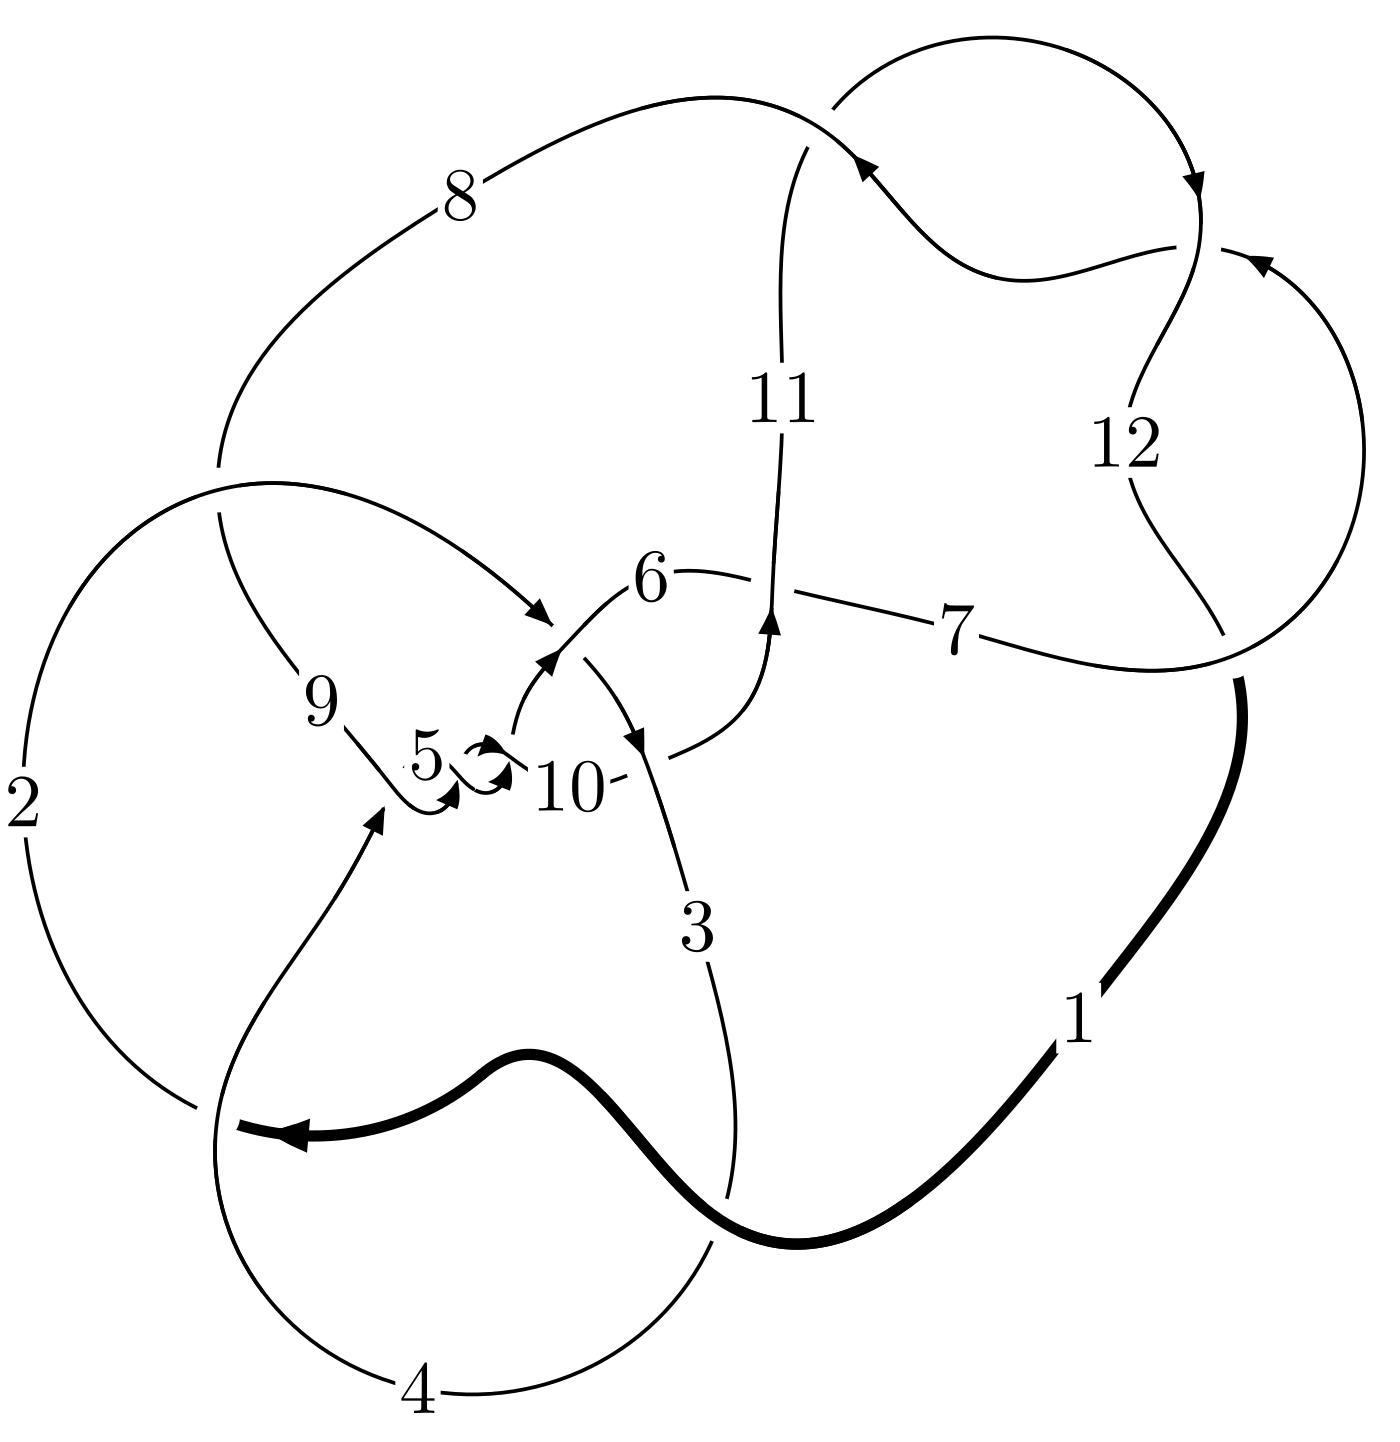
\includegraphics[width=112pt]{../../../GIT/diagram.site/Diagrams/png/1813_12a_1012.png}\\
\ \ \ A knot diagram\footnotemark}&
\allowdisplaybreaks
\textbf{Linearized knot diagam} \\
\cline{2-2}
 &
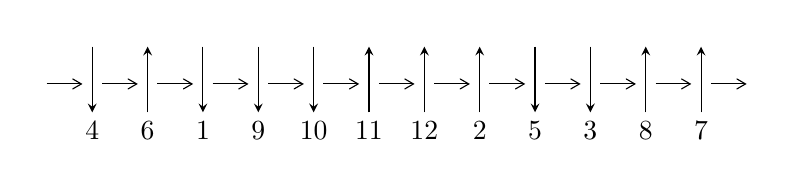
\begin{tikzpicture}[x=20pt, y=17pt]
	% nodes
	\node (C0) at (0, 0) {};
	\node (C1) at (1, 0) {};
	\node (C1U) at (1, +1) {};
	\node (C1D) at (1, -1) {4};

	\node (C2) at (2, 0) {};
	\node (C2U) at (2, +1) {};
	\node (C2D) at (2, -1) {6};

	\node (C3) at (3, 0) {};
	\node (C3U) at (3, +1) {};
	\node (C3D) at (3, -1) {1};

	\node (C4) at (4, 0) {};
	\node (C4U) at (4, +1) {};
	\node (C4D) at (4, -1) {9};

	\node (C5) at (5, 0) {};
	\node (C5U) at (5, +1) {};
	\node (C5D) at (5, -1) {10};

	\node (C6) at (6, 0) {};
	\node (C6U) at (6, +1) {};
	\node (C6D) at (6, -1) {11};

	\node (C7) at (7, 0) {};
	\node (C7U) at (7, +1) {};
	\node (C7D) at (7, -1) {12};

	\node (C8) at (8, 0) {};
	\node (C8U) at (8, +1) {};
	\node (C8D) at (8, -1) {2};

	\node (C9) at (9, 0) {};
	\node (C9U) at (9, +1) {};
	\node (C9D) at (9, -1) {5};

	\node (C10) at (10, 0) {};
	\node (C10U) at (10, +1) {};
	\node (C10D) at (10, -1) {3};

	\node (C11) at (11, 0) {};
	\node (C11U) at (11, +1) {};
	\node (C11D) at (11, -1) {8};

	\node (C12) at (12, 0) {};
	\node (C12U) at (12, +1) {};
	\node (C12D) at (12, -1) {7};
	\node (C13) at (13, 0) {};

	% arrows
	\draw[->,>={angle 60}]
	(C0) edge (C1) (C1) edge (C2) (C2) edge (C3) (C3) edge (C4) (C4) edge (C5) (C5) edge (C6) (C6) edge (C7) (C7) edge (C8) (C8) edge (C9) (C9) edge (C10) (C10) edge (C11) (C11) edge (C12) (C12) edge (C13) ;	\draw[->,>=stealth]
	(C1U) edge (C1D) (C2D) edge (C2U) (C3U) edge (C3D) (C4U) edge (C4D) (C5U) edge (C5D) (C6D) edge (C6U) (C7D) edge (C7U) (C8D) edge (C8U) (C9U) edge (C9D) (C10U) edge (C10D) (C11D) edge (C11U) (C12D) edge (C12U) ;
	\end{tikzpicture} \\
\hhline{~~} \\& 
\textbf{Solving Sequence} \\ \cline{2-2} 
 &
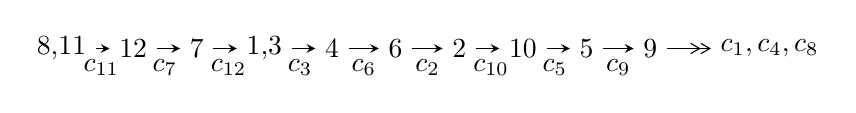
\begin{tikzpicture}[x=23pt, y=7pt]
	% node
	\node (A0) at (-1/8, 0) {8,11};
	\node (A1) at (1, 0) {12};
	\node (A2) at (2, 0) {7};
	\node (A3) at (49/16, 0) {1,3};
	\node (A4) at (33/8, 0) {4};
	\node (A5) at (41/8, 0) {6};
	\node (A6) at (49/8, 0) {2};
	\node (A7) at (57/8, 0) {10};
	\node (A8) at (65/8, 0) {5};
	\node (A9) at (73/8, 0) {9};
	\node (C1) at (1/2, -1) {$c_{11}$};
	\node (C2) at (3/2, -1) {$c_{7}$};
	\node (C3) at (5/2, -1) {$c_{12}$};
	\node (C4) at (29/8, -1) {$c_{3}$};
	\node (C5) at (37/8, -1) {$c_{6}$};
	\node (C6) at (45/8, -1) {$c_{2}$};
	\node (C7) at (53/8, -1) {$c_{10}$};
	\node (C8) at (61/8, -1) {$c_{5}$};
	\node (C9) at (69/8, -1) {$c_{9}$};
	\node (A10) at (11, 0) {$c_{1},c_{4},c_{8}$};

	% edge
	\draw[->,>=stealth]	
	(A0) edge (A1) (A1) edge (A2) (A2) edge (A3) (A3) edge (A4) (A4) edge (A5) (A5) edge (A6) (A6) edge (A7) (A7) edge (A8) (A8) edge (A9) ;
	\draw[->>,>={angle 60}]	
	(A9) edge (A10);
\end{tikzpicture} \\ 

\end{tabular} \\

\footnotetext{
The image of knot diagram is generated by the software ``\textbf{Draw programme}" developed by Andrew Bartholomew(\url{http://www.layer8.co.uk/maths/draw/index.htm\#Running-draw}), where we modified some parts for our purpose(\url{https://github.com/CATsTAILs/LinksPainter}).
}\phantom \\ \newline 
\centering \textbf{Ideals for irreducible components\footnotemark of $X_{\text{par}}$} 
 
\begin{align*}
I^u_{1}&=\langle 
-2.05532\times10^{66} u^{82}+2.51093\times10^{66} u^{81}+\cdots+1.60291\times10^{67} b-6.72720\times10^{65},\\
\phantom{I^u_{1}}&\phantom{= \langle  }1.11417\times10^{67} u^{82}-1.22744\times10^{67} u^{81}+\cdots+1.60291\times10^{67} a-2.52964\times10^{67},\;u^{83}-2 u^{82}+\cdots-2 u+1\rangle \\
I^u_{2}&=\langle 
7 b-2 u-1,\;7 a+u+4,\;u^2- u+1\rangle \\
\\
\end{align*}
\raggedright * 2 irreducible components of $\dim_{\mathbb{C}}=0$, with total 85 representations.\\
\footnotetext{All coefficients of polynomials are rational numbers. But the coefficients are sometimes approximated in decimal forms when there is not enough margin.}
\newpage
\renewcommand{\arraystretch}{1}
\centering \section*{I. $I^u_{1}= \langle -2.06\times10^{66} u^{82}+2.51\times10^{66} u^{81}+\cdots+1.60\times10^{67} b-6.73\times10^{65},\;1.11\times10^{67} u^{82}-1.23\times10^{67} u^{81}+\cdots+1.60\times10^{67} a-2.53\times10^{67},\;u^{83}-2 u^{82}+\cdots-2 u+1 \rangle$}
\flushleft \textbf{(i) Arc colorings}\\
\begin{tabular}{m{7pt} m{180pt} m{7pt} m{180pt} }
\flushright $a_{8}=$&$\begin{pmatrix}0\\u\end{pmatrix}$ \\
\flushright $a_{11}=$&$\begin{pmatrix}1\\0\end{pmatrix}$ \\
\flushright $a_{12}=$&$\begin{pmatrix}1\\- u^2\end{pmatrix}$ \\
\flushright $a_{7}=$&$\begin{pmatrix}- u\\u^3+u\end{pmatrix}$ \\
\flushright $a_{1}=$&$\begin{pmatrix}u^2+1\\- u^4-2 u^2\end{pmatrix}$ \\
\flushright $a_{3}=$&$\begin{pmatrix}-0.695089 u^{82}+0.765754 u^{81}+\cdots-0.805908 u+1.57815\\0.128224 u^{82}-0.156648 u^{81}+\cdots-0.183076 u+0.0419686\end{pmatrix}$ \\
\flushright $a_{4}=$&$\begin{pmatrix}-0.506927 u^{82}+0.383641 u^{81}+\cdots+0.301338 u+0.370054\\0.187208 u^{82}-0.231332 u^{81}+\cdots+0.176599 u+0.0714091\end{pmatrix}$ \\
\flushright $a_{6}=$&$\begin{pmatrix}- u^3-2 u\\u^3+u\end{pmatrix}$ \\
\flushright $a_{2}=$&$\begin{pmatrix}-0.771316 u^{82}+0.876988 u^{81}+\cdots-1.09248 u+1.44647\\0.168393 u^{82}-0.226519 u^{81}+\cdots-0.0270658 u+0.0924313\end{pmatrix}$ \\
\flushright $a_{10}=$&$\begin{pmatrix}2.08991 u^{82}-3.13988 u^{81}+\cdots-3.52603 u-2.11892\\-1.17284 u^{82}+1.89402 u^{81}+\cdots+3.09591 u+0.772956\end{pmatrix}$ \\
\flushright $a_{5}=$&$\begin{pmatrix}1.18628 u^{82}-3.04794 u^{81}+\cdots-5.78944 u+1.01993\\-0.959505 u^{82}+1.55012 u^{81}+\cdots+4.15771 u-0.726348\end{pmatrix}$ \\
\flushright $a_{9}=$&$\begin{pmatrix}1.32283 u^{82}-1.63143 u^{81}+\cdots+2.70703 u-4.79684\\-1.24263 u^{82}+0.911270 u^{81}+\cdots-0.275552 u+2.26730\end{pmatrix}$\\&\end{tabular}
\flushleft \textbf{(ii) Obstruction class $= -1$}\\~\\
\flushleft \textbf{(iii) Cusp Shapes $= -0.167112 u^{82}+1.45471 u^{81}+\cdots-2.64274 u+0.360927$}\\~\\
\newpage\renewcommand{\arraystretch}{1}
\flushleft \textbf{(iv) u-Polynomials at the component}\newline \\
\begin{tabular}{m{50pt}|m{274pt}}
Crossings & \hspace{64pt}u-Polynomials at each crossing \\
\hline $$\begin{aligned}c_{1},c_{3}\end{aligned}$$&$\begin{aligned}
&u^{83}-3 u^{82}+\cdots+285 u+49
\end{aligned}$\\
\hline $$\begin{aligned}c_{2}\end{aligned}$$&$\begin{aligned}
&u^{83}-7 u^{82}+\cdots+1260 u-196
\end{aligned}$\\
\hline $$\begin{aligned}c_{4},c_{5},c_{9}\end{aligned}$$&$\begin{aligned}
&u^{83}-2 u^{82}+\cdots+2 u^2-1
\end{aligned}$\\
\hline $$\begin{aligned}c_{6}\end{aligned}$$&$\begin{aligned}
&u^{83}+2 u^{82}+\cdots+762 u+65
\end{aligned}$\\
\hline $$\begin{aligned}c_{7},c_{11},c_{12}\end{aligned}$$&$\begin{aligned}
&u^{83}-2 u^{82}+\cdots-2 u+1
\end{aligned}$\\
\hline $$\begin{aligned}c_{8}\end{aligned}$$&$\begin{aligned}
&7(7 u^{83}+28 u^{82}+\cdots+4430074 u+1636183)
\end{aligned}$\\
\hline $$\begin{aligned}c_{10}\end{aligned}$$&$\begin{aligned}
&7(7 u^{83}-49 u^{82}+\cdots+141221 u-21311)
\end{aligned}$\\
\hline
\end{tabular}\\~\\
\newpage\renewcommand{\arraystretch}{1}
\flushleft \textbf{(v) Riley Polynomials at the component}\newline \\
\begin{tabular}{m{50pt}|m{274pt}}
Crossings & \hspace{64pt}Riley Polynomials at each crossing \\
\hline $$\begin{aligned}c_{1},c_{3}\end{aligned}$$&$\begin{aligned}
&y^{83}-63 y^{82}+\cdots-5505 y-2401
\end{aligned}$\\
\hline $$\begin{aligned}c_{2}\end{aligned}$$&$\begin{aligned}
&y^{83}+15 y^{82}+\cdots-873768 y-38416
\end{aligned}$\\
\hline $$\begin{aligned}c_{4},c_{5},c_{9}\end{aligned}$$&$\begin{aligned}
&y^{83}-84 y^{82}+\cdots+4 y-1
\end{aligned}$\\
\hline $$\begin{aligned}c_{6}\end{aligned}$$&$\begin{aligned}
&y^{83}-12 y^{82}+\cdots+353924 y-4225
\end{aligned}$\\
\hline $$\begin{aligned}c_{7},c_{11},c_{12}\end{aligned}$$&$\begin{aligned}
&y^{83}+72 y^{82}+\cdots+4 y-1
\end{aligned}$\\
\hline $$\begin{aligned}c_{8}\end{aligned}$$&$\begin{aligned}
&49\\
&\cdot(49 y^{83}+2716 y^{82}+\cdots-90553024520728 y-2677094809489)
\end{aligned}$\\
\hline $$\begin{aligned}c_{10}\end{aligned}$$&$\begin{aligned}
&49(49 y^{83}-371 y^{82}+\cdots+1.72569\times10^{10} y-4.54159\times10^{8})
\end{aligned}$\\
\hline
\end{tabular}\\~\\
\newpage\flushleft \textbf{(vi) Complex Volumes and Cusp Shapes}
$$\begin{array}{c|c|c}  
\text{Solutions to }I^u_{1}& \I (\text{vol} + \sqrt{-1}CS) & \text{Cusp shape}\\
 \hline 
\begin{aligned}
u &= \phantom{-}0.475006 + 0.859601 I \\
a &= \phantom{-}1.067640 - 0.053405 I \\
b &= -1.19843 - 0.84086 I\end{aligned}
 & -10.20070 - 8.08224 I & \phantom{-0.000000 } 0 \\ \hline\begin{aligned}
u &= \phantom{-}0.475006 - 0.859601 I \\
a &= \phantom{-}1.067640 + 0.053405 I \\
b &= -1.19843 + 0.84086 I\end{aligned}
 & -10.20070 + 8.08224 I & \phantom{-0.000000 } 0 \\ \hline\begin{aligned}
u &= \phantom{-}0.064627 + 1.021110 I \\
a &= -0.097879 - 0.830642 I \\
b &= \phantom{-}0.816969 + 0.914245 I\end{aligned}
 & -5.67104 - 3.00245 I & \phantom{-0.000000 } 0 \\ \hline\begin{aligned}
u &= \phantom{-}0.064627 - 1.021110 I \\
a &= -0.097879 + 0.830642 I \\
b &= \phantom{-}0.816969 - 0.914245 I\end{aligned}
 & -5.67104 + 3.00245 I & \phantom{-0.000000 } 0 \\ \hline\begin{aligned}
u &= -0.514621 + 0.829465 I \\
a &= \phantom{-}0.878968 - 0.069917 I \\
b &= -0.828395 + 0.694970 I\end{aligned}
 & -2.74113 + 4.19441 I & \phantom{-0.000000 } 0 \\ \hline\begin{aligned}
u &= -0.514621 - 0.829465 I \\
a &= \phantom{-}0.878968 + 0.069917 I \\
b &= -0.828395 - 0.694970 I\end{aligned}
 & -2.74113 - 4.19441 I & \phantom{-0.000000 } 0 \\ \hline\begin{aligned}
u &= -0.887144 + 0.240007 I \\
a &= -0.903715 - 0.450278 I \\
b &= \phantom{-}0.644498 - 0.077979 I\end{aligned}
 & -7.32946 + 1.81939 I & -9.08409 - 3.25302 I \\ \hline\begin{aligned}
u &= -0.887144 - 0.240007 I \\
a &= -0.903715 + 0.450278 I \\
b &= \phantom{-}0.644498 + 0.077979 I\end{aligned}
 & -7.32946 - 1.81939 I & -9.08409 + 3.25302 I \\ \hline\begin{aligned}
u &= -0.196848 + 1.067180 I \\
a &= -0.135156 + 0.515710 I \\
b &= \phantom{-}0.433799 - 0.853225 I\end{aligned}
 & \phantom{-}0.117492 + 0.387913 I & \phantom{-0.000000 } 0 \\ \hline\begin{aligned}
u &= -0.196848 - 1.067180 I \\
a &= -0.135156 - 0.515710 I \\
b &= \phantom{-}0.433799 + 0.853225 I\end{aligned}
 & \phantom{-}0.117492 - 0.387913 I & \phantom{-0.000000 } 0\\
 \hline 
 \end{array}$$\newpage$$\begin{array}{c|c|c}  
\text{Solutions to }I^u_{1}& \I (\text{vol} + \sqrt{-1}CS) & \text{Cusp shape}\\
 \hline 
\begin{aligned}
u &= -0.485786 + 0.988027 I \\
a &= \phantom{-}0.446200 + 0.372854 I \\
b &= -0.791315 - 0.421140 I\end{aligned}
 & -9.68489 - 6.70543 I & \phantom{-0.000000 } 0 \\ \hline\begin{aligned}
u &= -0.485786 - 0.988027 I \\
a &= \phantom{-}0.446200 - 0.372854 I \\
b &= -0.791315 + 0.421140 I\end{aligned}
 & -9.68489 + 6.70543 I & \phantom{-0.000000 } 0 \\ \hline\begin{aligned}
u &= \phantom{-}0.831753 + 0.330980 I \\
a &= -0.300588 + 1.183040 I \\
b &= \phantom{-}0.605846 - 0.630936 I\end{aligned}
 & -0.32503 + 3.27303 I & -2.53912 - 7.98791 I \\ \hline\begin{aligned}
u &= \phantom{-}0.831753 - 0.330980 I \\
a &= -0.300588 - 1.183040 I \\
b &= \phantom{-}0.605846 + 0.630936 I\end{aligned}
 & -0.32503 - 3.27303 I & -2.53912 + 7.98791 I \\ \hline\begin{aligned}
u &= \phantom{-}0.648808 + 0.920395 I \\
a &= \phantom{-}0.494724 + 0.001353 I \\
b &= -0.506519 - 0.199456 I\end{aligned}
 & -1.94282 + 1.87194 I & \phantom{-0.000000 } 0 \\ \hline\begin{aligned}
u &= \phantom{-}0.648808 - 0.920395 I \\
a &= \phantom{-}0.494724 - 0.001353 I \\
b &= -0.506519 + 0.199456 I\end{aligned}
 & -1.94282 - 1.87194 I & \phantom{-0.000000 } 0 \\ \hline\begin{aligned}
u &= -0.804514 + 0.287110 I \\
a &= -0.53594 - 1.81584 I \\
b &= \phantom{-}1.012310 + 0.946985 I\end{aligned}
 & -1.01980 - 8.80520 I & -1.34312 + 8.67899 I \\ \hline\begin{aligned}
u &= -0.804514 - 0.287110 I \\
a &= -0.53594 + 1.81584 I \\
b &= \phantom{-}1.012310 - 0.946985 I\end{aligned}
 & -1.01980 + 8.80520 I & -1.34312 - 8.67899 I \\ \hline\begin{aligned}
u &= \phantom{-}0.805730 + 0.269407 I \\
a &= -0.86968 + 2.12116 I \\
b &= \phantom{-}1.36813 - 1.02151 I\end{aligned}
 & -8.3267 + 12.6232 I & -3.82071 - 7.57574 I \\ \hline\begin{aligned}
u &= \phantom{-}0.805730 - 0.269407 I \\
a &= -0.86968 - 2.12116 I \\
b &= \phantom{-}1.36813 + 1.02151 I\end{aligned}
 & -8.3267 - 12.6232 I & -3.82071 + 7.57574 I\\
 \hline 
 \end{array}$$\newpage$$\begin{array}{c|c|c}  
\text{Solutions to }I^u_{1}& \I (\text{vol} + \sqrt{-1}CS) & \text{Cusp shape}\\
 \hline 
\begin{aligned}
u &= \phantom{-}0.315485 + 1.137810 I \\
a &= \phantom{-}0.011028 - 0.251257 I \\
b &= \phantom{-}0.149783 + 0.594962 I\end{aligned}
 & -0.96189 + 3.32369 I & \phantom{-0.000000 } 0 \\ \hline\begin{aligned}
u &= \phantom{-}0.315485 - 1.137810 I \\
a &= \phantom{-}0.011028 + 0.251257 I \\
b &= \phantom{-}0.149783 - 0.594962 I\end{aligned}
 & -0.96189 - 3.32369 I & \phantom{-0.000000 } 0 \\ \hline\begin{aligned}
u &= \phantom{-}0.721078 + 0.104434 I \\
a &= \phantom{-}0.192013 - 0.856291 I \\
b &= -0.541096 + 0.418060 I\end{aligned}
 & \phantom{-}2.18731 + 0.45631 I & \phantom{-}4.25707 + 1.46675 I \\ \hline\begin{aligned}
u &= \phantom{-}0.721078 - 0.104434 I \\
a &= \phantom{-}0.192013 + 0.856291 I \\
b &= -0.541096 - 0.418060 I\end{aligned}
 & \phantom{-}2.18731 - 0.45631 I & \phantom{-}4.25707 - 1.46675 I \\ \hline\begin{aligned}
u &= \phantom{-}0.697920 + 0.208237 I \\
a &= -0.06509 - 2.19317 I \\
b &= -1.001020 + 0.864477 I\end{aligned}
 & -3.51395 + 6.33078 I & -1.40613 - 6.95376 I \\ \hline\begin{aligned}
u &= \phantom{-}0.697920 - 0.208237 I \\
a &= -0.06509 + 2.19317 I \\
b &= -1.001020 - 0.864477 I\end{aligned}
 & -3.51395 - 6.33078 I & -1.40613 + 6.95376 I \\ \hline\begin{aligned}
u &= -0.705904 + 0.173366 I \\
a &= -0.00653 + 1.68655 I \\
b &= -0.751506 - 0.750263 I\end{aligned}
 & \phantom{-}2.69458 - 3.85814 I & \phantom{-}3.94212 + 7.39409 I \\ \hline\begin{aligned}
u &= -0.705904 - 0.173366 I \\
a &= -0.00653 - 1.68655 I \\
b &= -0.751506 + 0.750263 I\end{aligned}
 & \phantom{-}2.69458 + 3.85814 I & \phantom{-}3.94212 - 7.39409 I \\ \hline\begin{aligned}
u &= -0.201198 + 1.284730 I \\
a &= -5.05419 + 0.23869 I \\
b &= \phantom{-}0.47343 - 6.07002 I\end{aligned}
 & -9.49174 - 2.91911 I & \phantom{-0.000000 } 0 \\ \hline\begin{aligned}
u &= -0.201198 - 1.284730 I \\
a &= -5.05419 - 0.23869 I \\
b &= \phantom{-}0.47343 + 6.07002 I\end{aligned}
 & -9.49174 + 2.91911 I & \phantom{-0.000000 } 0\\
 \hline 
 \end{array}$$\newpage$$\begin{array}{c|c|c}  
\text{Solutions to }I^u_{1}& \I (\text{vol} + \sqrt{-1}CS) & \text{Cusp shape}\\
 \hline 
\begin{aligned}
u &= \phantom{-}0.153067 + 1.295210 I \\
a &= -1.46523 - 0.72615 I \\
b &= -0.708458 + 1.122390 I\end{aligned}
 & -4.25517 + 1.80505 I & \phantom{-0.000000 } 0 \\ \hline\begin{aligned}
u &= \phantom{-}0.153067 - 1.295210 I \\
a &= -1.46523 + 0.72615 I \\
b &= -0.708458 - 1.122390 I\end{aligned}
 & -4.25517 - 1.80505 I & \phantom{-0.000000 } 0 \\ \hline\begin{aligned}
u &= -0.103113 + 1.315490 I \\
a &= -1.137520 + 0.803248 I \\
b &= -0.446110 - 0.029511 I\end{aligned}
 & -4.75098 + 0.70977 I & \phantom{-0.000000 } 0 \\ \hline\begin{aligned}
u &= -0.103113 - 1.315490 I \\
a &= -1.137520 - 0.803248 I \\
b &= -0.446110 + 0.029511 I\end{aligned}
 & -4.75098 - 0.70977 I & \phantom{-0.000000 } 0 \\ \hline\begin{aligned}
u &= -0.246151 + 1.332300 I \\
a &= -0.65866 - 1.28463 I \\
b &= \phantom{-}1.63452 - 0.64490 I\end{aligned}
 & -8.26726 - 2.71936 I & \phantom{-0.000000 } 0 \\ \hline\begin{aligned}
u &= -0.246151 - 1.332300 I \\
a &= -0.65866 + 1.28463 I \\
b &= \phantom{-}1.63452 + 0.64490 I\end{aligned}
 & -8.26726 + 2.71936 I & \phantom{-0.000000 } 0 \\ \hline\begin{aligned}
u &= \phantom{-}0.214045 + 1.342100 I \\
a &= \phantom{-}1.45885 + 0.68329 I \\
b &= -0.32165 - 2.41633 I\end{aligned}
 & -5.15605 + 3.28846 I & \phantom{-0.000000 } 0 \\ \hline\begin{aligned}
u &= \phantom{-}0.214045 - 1.342100 I \\
a &= \phantom{-}1.45885 - 0.68329 I \\
b &= -0.32165 + 2.41633 I\end{aligned}
 & -5.15605 - 3.28846 I & \phantom{-0.000000 } 0 \\ \hline\begin{aligned}
u &= \phantom{-}0.088800 + 1.356500 I \\
a &= -1.27024 - 0.97335 I \\
b &= -0.624479 - 0.521635 I\end{aligned}
 & -11.14690 - 2.43409 I & \phantom{-0.000000 } 0 \\ \hline\begin{aligned}
u &= \phantom{-}0.088800 - 1.356500 I \\
a &= -1.27024 + 0.97335 I \\
b &= -0.624479 + 0.521635 I\end{aligned}
 & -11.14690 + 2.43409 I & \phantom{-0.000000 } 0\\
 \hline 
 \end{array}$$\newpage$$\begin{array}{c|c|c}  
\text{Solutions to }I^u_{1}& \I (\text{vol} + \sqrt{-1}CS) & \text{Cusp shape}\\
 \hline 
\begin{aligned}
u &= \phantom{-}0.283140 + 1.336130 I \\
a &= \phantom{-}0.505201 + 0.841714 I \\
b &= \phantom{-}0.890946 - 0.298623 I\end{aligned}
 & -2.35239 + 4.06574 I & \phantom{-0.000000 } 0 \\ \hline\begin{aligned}
u &= \phantom{-}0.283140 - 1.336130 I \\
a &= \phantom{-}0.505201 - 0.841714 I \\
b &= \phantom{-}0.890946 + 0.298623 I\end{aligned}
 & -2.35239 - 4.06574 I & \phantom{-0.000000 } 0 \\ \hline\begin{aligned}
u &= -0.176964 + 1.360150 I \\
a &= -0.590958 + 0.069979 I \\
b &= -1.215720 + 0.395720 I\end{aligned}
 & -7.28744 - 1.94916 I & \phantom{-0.000000 } 0 \\ \hline\begin{aligned}
u &= -0.176964 - 1.360150 I \\
a &= -0.590958 - 0.069979 I \\
b &= -1.215720 - 0.395720 I\end{aligned}
 & -7.28744 + 1.94916 I & \phantom{-0.000000 } 0 \\ \hline\begin{aligned}
u &= \phantom{-}0.562967 + 0.258206 I \\
a &= \phantom{-}0.91272 - 2.17851 I \\
b &= -0.502187 - 0.190942 I\end{aligned}
 & -8.27455 + 3.42400 I & -6.60317 - 6.41709 I \\ \hline\begin{aligned}
u &= \phantom{-}0.562967 - 0.258206 I \\
a &= \phantom{-}0.91272 + 2.17851 I \\
b &= -0.502187 + 0.190942 I\end{aligned}
 & -8.27455 - 3.42400 I & -6.60317 + 6.41709 I \\ \hline\begin{aligned}
u &= -0.593523 + 0.159631 I \\
a &= \phantom{-}2.10426 - 0.35004 I \\
b &= -1.068470 + 0.631484 I\end{aligned}
 & -3.63121 + 0.36859 I & \phantom{-}0.14544 + 2.24269 I \\ \hline\begin{aligned}
u &= -0.593523 - 0.159631 I \\
a &= \phantom{-}2.10426 + 0.35004 I \\
b &= -1.068470 - 0.631484 I\end{aligned}
 & -3.63121 - 0.36859 I & \phantom{-}0.14544 - 2.24269 I \\ \hline\begin{aligned}
u &= -0.227049 + 1.369170 I \\
a &= \phantom{-}0.45671 - 1.47672 I \\
b &= \phantom{-}0.458092 + 0.749861 I\end{aligned}
 & -6.58085 - 5.34361 I & \phantom{-0.000000 } 0 \\ \hline\begin{aligned}
u &= -0.227049 - 1.369170 I \\
a &= \phantom{-}0.45671 + 1.47672 I \\
b &= \phantom{-}0.458092 - 0.749861 I\end{aligned}
 & -6.58085 + 5.34361 I & \phantom{-0.000000 } 0\\
 \hline 
 \end{array}$$\newpage$$\begin{array}{c|c|c}  
\text{Solutions to }I^u_{1}& \I (\text{vol} + \sqrt{-1}CS) & \text{Cusp shape}\\
 \hline 
\begin{aligned}
u &= -0.612038\phantom{ +0.000000I} \\
a &= \phantom{-}13.8516\phantom{ +0.000000I} \\
b &= -8.20930\phantom{ +0.000000I}\end{aligned}
 & -5.55052\phantom{ +0.000000I} & \phantom{-}56.4320\phantom{ +0.000000I} \\ \hline\begin{aligned}
u &= \phantom{-}0.024059 + 0.608715 I \\
a &= \phantom{-}0.522848 - 0.442561 I \\
b &= \phantom{-}0.816972 + 0.871424 I\end{aligned}
 & -5.56598 - 3.04650 I & -5.26168 + 2.94884 I \\ \hline\begin{aligned}
u &= \phantom{-}0.024059 - 0.608715 I \\
a &= \phantom{-}0.522848 + 0.442561 I \\
b &= \phantom{-}0.816972 - 0.871424 I\end{aligned}
 & -5.56598 + 3.04650 I & -5.26168 - 2.94884 I \\ \hline\begin{aligned}
u &= -0.284196 + 1.364560 I \\
a &= \phantom{-}1.05657 - 1.05386 I \\
b &= \phantom{-}0.944479 + 0.673054 I\end{aligned}
 & -2.17553 - 7.44915 I & \phantom{-0.000000 } 0 \\ \hline\begin{aligned}
u &= -0.284196 - 1.364560 I \\
a &= \phantom{-}1.05657 + 1.05386 I \\
b &= \phantom{-}0.944479 - 0.673054 I\end{aligned}
 & -2.17553 + 7.44915 I & \phantom{-0.000000 } 0 \\ \hline\begin{aligned}
u &= \phantom{-}0.171165 + 1.383490 I \\
a &= -1.236300 + 0.358353 I \\
b &= -1.122770 - 0.073322 I\end{aligned}
 & -14.2618 + 1.5244 I & \phantom{-0.000000 } 0 \\ \hline\begin{aligned}
u &= \phantom{-}0.171165 - 1.383490 I \\
a &= -1.236300 - 0.358353 I \\
b &= -1.122770 + 0.073322 I\end{aligned}
 & -14.2618 - 1.5244 I & \phantom{-0.000000 } 0 \\ \hline\begin{aligned}
u &= \phantom{-}0.226585 + 1.387380 I \\
a &= \phantom{-}0.14113 + 1.87100 I \\
b &= \phantom{-}0.487387 - 0.142506 I\end{aligned}
 & -13.4949 + 6.3486 I & \phantom{-0.000000 } 0 \\ \hline\begin{aligned}
u &= \phantom{-}0.226585 - 1.387380 I \\
a &= \phantom{-}0.14113 - 1.87100 I \\
b &= \phantom{-}0.487387 + 0.142506 I\end{aligned}
 & -13.4949 - 6.3486 I & \phantom{-0.000000 } 0 \\ \hline\begin{aligned}
u &= \phantom{-}0.280416 + 1.379490 I \\
a &= \phantom{-}1.37093 + 1.32206 I \\
b &= \phantom{-}1.109010 - 0.804345 I\end{aligned}
 & -8.55319 + 9.88755 I & \phantom{-0.000000 } 0\\
 \hline 
 \end{array}$$\newpage$$\begin{array}{c|c|c}  
\text{Solutions to }I^u_{1}& \I (\text{vol} + \sqrt{-1}CS) & \text{Cusp shape}\\
 \hline 
\begin{aligned}
u &= \phantom{-}0.280416 - 1.379490 I \\
a &= \phantom{-}1.37093 - 1.32206 I \\
b &= \phantom{-}1.109010 + 0.804345 I\end{aligned}
 & -8.55319 - 9.88755 I & \phantom{-0.000000 } 0 \\ \hline\begin{aligned}
u &= -0.556007 + 0.198624 I \\
a &= \phantom{-}0.64889 + 2.30970 I \\
b &= -0.361053 - 0.390068 I\end{aligned}
 & -1.60606 - 2.43462 I & -4.11520 + 8.58615 I \\ \hline\begin{aligned}
u &= -0.556007 - 0.198624 I \\
a &= \phantom{-}0.64889 - 2.30970 I \\
b &= -0.361053 + 0.390068 I\end{aligned}
 & -1.60606 + 2.43462 I & -4.11520 - 8.58615 I \\ \hline\begin{aligned}
u &= \phantom{-}0.540026 + 0.095845 I \\
a &= -0.08882 - 4.08497 I \\
b &= \phantom{-}0.11563 + 1.93050 I\end{aligned}
 & -0.576070 + 0.516826 I & \phantom{-}3.2266 + 14.4230 I \\ \hline\begin{aligned}
u &= \phantom{-}0.540026 - 0.095845 I \\
a &= -0.08882 + 4.08497 I \\
b &= \phantom{-}0.11563 - 1.93050 I\end{aligned}
 & -0.576070 - 0.516826 I & \phantom{-}3.2266 - 14.4230 I \\ \hline\begin{aligned}
u &= \phantom{-}0.32617 + 1.41892 I \\
a &= -0.77942 - 1.59755 I \\
b &= -1.52531 + 1.07291 I\end{aligned}
 & -13.7023 + 16.7170 I & \phantom{-0.000000 } 0 \\ \hline\begin{aligned}
u &= \phantom{-}0.32617 - 1.41892 I \\
a &= -0.77942 + 1.59755 I \\
b &= -1.52531 - 1.07291 I\end{aligned}
 & -13.7023 - 16.7170 I & \phantom{-0.000000 } 0 \\ \hline\begin{aligned}
u &= -0.32343 + 1.42557 I \\
a &= -0.73068 + 1.30369 I \\
b &= -1.19487 - 1.02795 I\end{aligned}
 & -6.4767 - 12.8862 I & \phantom{-0.000000 } 0 \\ \hline\begin{aligned}
u &= -0.32343 - 1.42557 I \\
a &= -0.73068 - 1.30369 I \\
b &= -1.19487 + 1.02795 I\end{aligned}
 & -6.4767 + 12.8862 I & \phantom{-0.000000 } 0 \\ \hline\begin{aligned}
u &= \phantom{-}0.32635 + 1.44037 I \\
a &= -0.511432 - 0.981821 I \\
b &= -0.839069 + 0.790583 I\end{aligned}
 & -5.96457 + 7.44234 I & \phantom{-0.000000 } 0\\
 \hline 
 \end{array}$$\newpage$$\begin{array}{c|c|c}  
\text{Solutions to }I^u_{1}& \I (\text{vol} + \sqrt{-1}CS) & \text{Cusp shape}\\
 \hline 
\begin{aligned}
u &= \phantom{-}0.32635 - 1.44037 I \\
a &= -0.511432 + 0.981821 I \\
b &= -0.839069 - 0.790583 I\end{aligned}
 & -5.96457 - 7.44234 I & \phantom{-0.000000 } 0 \\ \hline\begin{aligned}
u &= -0.35997 + 1.43695 I \\
a &= \phantom{-}0.040198 + 0.863532 I \\
b &= -0.714170 - 0.214535 I\end{aligned}
 & -12.69990 - 2.69645 I & \phantom{-0.000000 } 0 \\ \hline\begin{aligned}
u &= -0.35997 - 1.43695 I \\
a &= \phantom{-}0.040198 - 0.863532 I \\
b &= -0.714170 + 0.214535 I\end{aligned}
 & -12.69990 + 2.69645 I & \phantom{-0.000000 } 0 \\ \hline\begin{aligned}
u &= \phantom{-}0.363932 + 0.344823 I \\
a &= \phantom{-}0.666144 - 0.751661 I \\
b &= \phantom{-}1.099950 - 0.265568 I\end{aligned}
 & -8.91963 - 0.57767 I & -8.53729 - 2.31769 I \\ \hline\begin{aligned}
u &= \phantom{-}0.363932 - 0.344823 I \\
a &= \phantom{-}0.666144 + 0.751661 I \\
b &= \phantom{-}1.099950 + 0.265568 I\end{aligned}
 & -8.91963 + 0.57767 I & -8.53729 + 2.31769 I \\ \hline\begin{aligned}
u &= \phantom{-}0.01649 + 1.50014 I \\
a &= \phantom{-}0.405278 + 0.345940 I \\
b &= \phantom{-}1.39329 + 0.42487 I\end{aligned}
 & -18.0876 - 7.1086 I & \phantom{-0.000000 } 0 \\ \hline\begin{aligned}
u &= \phantom{-}0.01649 - 1.50014 I \\
a &= \phantom{-}0.405278 - 0.345940 I \\
b &= \phantom{-}1.39329 - 0.42487 I\end{aligned}
 & -18.0876 + 7.1086 I & \phantom{-0.000000 } 0 \\ \hline\begin{aligned}
u &= -0.01547 + 1.51995 I \\
a &= \phantom{-}0.229511 - 0.148482 I \\
b &= \phantom{-}1.151530 - 0.202710 I\end{aligned}
 & -10.80190 + 2.92909 I & \phantom{-0.000000 } 0 \\ \hline\begin{aligned}
u &= -0.01547 - 1.51995 I \\
a &= \phantom{-}0.229511 + 0.148482 I \\
b &= \phantom{-}1.151530 + 0.202710 I\end{aligned}
 & -10.80190 - 2.92909 I & \phantom{-0.000000 } 0 \\ \hline\begin{aligned}
u &= \phantom{-}0.146993 + 0.405037 I \\
a &= \phantom{-}0.805858 + 0.297081 I \\
b &= \phantom{-}0.282795 - 0.494464 I\end{aligned}
 & \phantom{-}0.039086 + 0.986146 I & \phantom{-}0.86398 - 6.49458 I\\
 \hline 
 \end{array}$$\newpage$$\begin{array}{c|c|c}  
\text{Solutions to }I^u_{1}& \I (\text{vol} + \sqrt{-1}CS) & \text{Cusp shape}\\
 \hline 
\begin{aligned}
u &= \phantom{-}0.146993 - 0.405037 I \\
a &= \phantom{-}0.805858 - 0.297081 I \\
b &= \phantom{-}0.282795 + 0.494464 I\end{aligned}
 & \phantom{-}0.039086 - 0.986146 I & \phantom{-}0.86398 + 6.49458 I \\ \hline\begin{aligned}
u &= -0.296698 + 0.219856 I \\
a &= \phantom{-}0.096577 + 0.687464 I \\
b &= \phantom{-}0.977900 - 0.039618 I\end{aligned}
 & -2.38293 + 0.13615 I & -6.35328 + 3.24648 I \\ \hline\begin{aligned}
u &= -0.296698 - 0.219856 I \\
a &= \phantom{-}0.096577 - 0.687464 I \\
b &= \phantom{-}0.977900 + 0.039618 I\end{aligned}
 & -2.38293 - 0.13615 I & -6.35328 - 3.24648 I\\
 \hline 
 \end{array}$$\newpage\newpage\renewcommand{\arraystretch}{1}
\centering \section*{II. $I^u_{2}= \langle 7 b-2 u-1,\;7 a+u+4,\;u^2- u+1 \rangle$}
\flushleft \textbf{(i) Arc colorings}\\
\begin{tabular}{m{7pt} m{180pt} m{7pt} m{180pt} }
\flushright $a_{8}=$&$\begin{pmatrix}0\\u\end{pmatrix}$ \\
\flushright $a_{11}=$&$\begin{pmatrix}1\\0\end{pmatrix}$ \\
\flushright $a_{12}=$&$\begin{pmatrix}1\\- u+1\end{pmatrix}$ \\
\flushright $a_{7}=$&$\begin{pmatrix}- u\\u-1\end{pmatrix}$ \\
\flushright $a_{1}=$&$\begin{pmatrix}u\\- u+2\end{pmatrix}$ \\
\flushright $a_{3}=$&$\begin{pmatrix}-\frac{1}{7} u-\frac{4}{7}\\\frac{2}{7} u+\frac{1}{7}\end{pmatrix}$ \\
\flushright $a_{4}=$&$\begin{pmatrix}-\frac{8}{7} u-\frac{4}{7}\\\frac{9}{7} u-\frac{13}{7}\end{pmatrix}$ \\
\flushright $a_{6}=$&$\begin{pmatrix}-2 u+1\\u-1\end{pmatrix}$ \\
\flushright $a_{2}=$&$\begin{pmatrix}-\frac{1}{7} u-\frac{4}{7}\\\frac{2}{7} u+\frac{1}{7}\end{pmatrix}$ \\
\flushright $a_{10}=$&$\begin{pmatrix}\frac{11}{49} u+\frac{51}{49}\\-\frac{8}{49} u+\frac{3}{49}\end{pmatrix}$ \\
\flushright $a_{5}=$&$\begin{pmatrix}-\frac{47}{49} u-\frac{13}{49}\\\frac{52}{49} u-\frac{44}{49}\end{pmatrix}$ \\
\flushright $a_{9}=$&$\begin{pmatrix}\frac{24}{49} u-\frac{9}{49}\\\frac{36}{49} u+\frac{11}{49}\end{pmatrix}$\\&\end{tabular}
\flushleft \textbf{(ii) Obstruction class $= 1$}\\~\\
\flushleft \textbf{(iii) Cusp Shapes $= -\frac{340}{49} u+\frac{299}{49}$}\\~\\
\newpage\renewcommand{\arraystretch}{1}
\flushleft \textbf{(iv) u-Polynomials at the component}\newline \\
\begin{tabular}{m{50pt}|m{274pt}}
Crossings & \hspace{64pt}u-Polynomials at each crossing \\
\hline $$\begin{aligned}c_{1}\end{aligned}$$&$\begin{aligned}
&(u-1)^2
\end{aligned}$\\
\hline $$\begin{aligned}c_{2}\end{aligned}$$&$\begin{aligned}
&u^2
\end{aligned}$\\
\hline $$\begin{aligned}c_{3}\end{aligned}$$&$\begin{aligned}
&(u+1)^2
\end{aligned}$\\
\hline $$\begin{aligned}c_{4},c_{5},c_{6}\\c_{11},c_{12}\end{aligned}$$&$\begin{aligned}
&u^2- u+1
\end{aligned}$\\
\hline $$\begin{aligned}c_{7},c_{9}\end{aligned}$$&$\begin{aligned}
&u^2+u+1
\end{aligned}$\\
\hline $$\begin{aligned}c_{8}\end{aligned}$$&$\begin{aligned}
&7(7 u^2-3 u+3)
\end{aligned}$\\
\hline $$\begin{aligned}c_{10}\end{aligned}$$&$\begin{aligned}
&7(7 u^2-4 u+1)
\end{aligned}$\\
\hline
\end{tabular}\\~\\
\newpage\renewcommand{\arraystretch}{1}
\flushleft \textbf{(v) Riley Polynomials at the component}\newline \\
\begin{tabular}{m{50pt}|m{274pt}}
Crossings & \hspace{64pt}Riley Polynomials at each crossing \\
\hline $$\begin{aligned}c_{1},c_{3}\end{aligned}$$&$\begin{aligned}
&(y-1)^2
\end{aligned}$\\
\hline $$\begin{aligned}c_{2}\end{aligned}$$&$\begin{aligned}
&y^2
\end{aligned}$\\
\hline $$\begin{aligned}c_{4},c_{5},c_{6}\\c_{7},c_{9},c_{11}\\c_{12}\end{aligned}$$&$\begin{aligned}
&y^2+y+1
\end{aligned}$\\
\hline $$\begin{aligned}c_{8}\end{aligned}$$&$\begin{aligned}
&49(49 y^2+33 y+9)
\end{aligned}$\\
\hline $$\begin{aligned}c_{10}\end{aligned}$$&$\begin{aligned}
&49(49 y^2-2 y+1)
\end{aligned}$\\
\hline
\end{tabular}\\~\\
\newpage\flushleft \textbf{(vi) Complex Volumes and Cusp Shapes}
$$\begin{array}{c|c|c}  
\text{Solutions to }I^u_{2}& \I (\text{vol} + \sqrt{-1}CS) & \text{Cusp shape}\\
 \hline 
\begin{aligned}
u &= \phantom{-}0.500000 + 0.866025 I \\
a &= -0.642857 - 0.123718 I \\
b &= \phantom{-}0.285714 + 0.247436 I\end{aligned}
 & -1.64493 + 2.02988 I & \phantom{-}2.63265 - 6.00916 I \\ \hline\begin{aligned}
u &= \phantom{-}0.500000 - 0.866025 I \\
a &= -0.642857 + 0.123718 I \\
b &= \phantom{-}0.285714 - 0.247436 I\end{aligned}
 & -1.64493 - 2.02988 I & \phantom{-}2.63265 + 6.00916 I\\
 \hline 
 \end{array}$$\newpage
\newpage\renewcommand{\arraystretch}{1}
\centering \section*{ III. u-Polynomials}
\begin{tabular}{m{50pt}|m{274pt}}
Crossings & \hspace{64pt}u-Polynomials at each crossing \\
\hline $$\begin{aligned}c_{1}\end{aligned}$$&$\begin{aligned}
&((u-1)^2)(u^{83}-3 u^{82}+\cdots+285 u+49)
\end{aligned}$\\
\hline $$\begin{aligned}c_{2}\end{aligned}$$&$\begin{aligned}
&u^2(u^{83}-7 u^{82}+\cdots+1260 u-196)
\end{aligned}$\\
\hline $$\begin{aligned}c_{3}\end{aligned}$$&$\begin{aligned}
&((u+1)^2)(u^{83}-3 u^{82}+\cdots+285 u+49)
\end{aligned}$\\
\hline $$\begin{aligned}c_{4},c_{5}\end{aligned}$$&$\begin{aligned}
&(u^2- u+1)(u^{83}-2 u^{82}+\cdots+2 u^2-1)
\end{aligned}$\\
\hline $$\begin{aligned}c_{6}\end{aligned}$$&$\begin{aligned}
&(u^2- u+1)(u^{83}+2 u^{82}+\cdots+762 u+65)
\end{aligned}$\\
\hline $$\begin{aligned}c_{7}\end{aligned}$$&$\begin{aligned}
&(u^2+u+1)(u^{83}-2 u^{82}+\cdots-2 u+1)
\end{aligned}$\\
\hline $$\begin{aligned}c_{8}\end{aligned}$$&$\begin{aligned}
&49(7 u^2-3 u+3)(7 u^{83}+28 u^{82}+\cdots+4430074 u+1636183)
\end{aligned}$\\
\hline $$\begin{aligned}c_{9}\end{aligned}$$&$\begin{aligned}
&(u^2+u+1)(u^{83}-2 u^{82}+\cdots+2 u^2-1)
\end{aligned}$\\
\hline $$\begin{aligned}c_{10}\end{aligned}$$&$\begin{aligned}
&49(7 u^2-4 u+1)(7 u^{83}-49 u^{82}+\cdots+141221 u-21311)
\end{aligned}$\\
\hline $$\begin{aligned}c_{11},c_{12}\end{aligned}$$&$\begin{aligned}
&(u^2- u+1)(u^{83}-2 u^{82}+\cdots-2 u+1)
\end{aligned}$\\
\hline
\end{tabular}\newpage\renewcommand{\arraystretch}{1}
\centering \section*{ IV. Riley Polynomials}
\begin{tabular}{m{50pt}|m{274pt}}
Crossings & \hspace{64pt}Riley Polynomials at each crossing \\
\hline $$\begin{aligned}c_{1},c_{3}\end{aligned}$$&$\begin{aligned}
&((y-1)^2)(y^{83}-63 y^{82}+\cdots-5505 y-2401)
\end{aligned}$\\
\hline $$\begin{aligned}c_{2}\end{aligned}$$&$\begin{aligned}
&y^2(y^{83}+15 y^{82}+\cdots-873768 y-38416)
\end{aligned}$\\
\hline $$\begin{aligned}c_{4},c_{5},c_{9}\end{aligned}$$&$\begin{aligned}
&(y^2+y+1)(y^{83}-84 y^{82}+\cdots+4 y-1)
\end{aligned}$\\
\hline $$\begin{aligned}c_{6}\end{aligned}$$&$\begin{aligned}
&(y^2+y+1)(y^{83}-12 y^{82}+\cdots+353924 y-4225)
\end{aligned}$\\
\hline $$\begin{aligned}c_{7},c_{11},c_{12}\end{aligned}$$&$\begin{aligned}
&(y^2+y+1)(y^{83}+72 y^{82}+\cdots+4 y-1)
\end{aligned}$\\
\hline $$\begin{aligned}c_{8}\end{aligned}$$&$\begin{aligned}
&2401(49 y^2+33 y+9)\\
&\cdot(49 y^{83}+2716 y^{82}+\cdots-90553024520728 y-2677094809489)
\end{aligned}$\\
\hline $$\begin{aligned}c_{10}\end{aligned}$$&$\begin{aligned}
&2401(49 y^2-2 y+1)\\
&\cdot(49 y^{83}-371 y^{82}+\cdots+17256948803 y-454158721)
\end{aligned}$\\
\hline
\end{tabular}
\vskip 2pc
\end{document}